\procTitle{Моделирование электрических цепей постоянного тока}
\procAuthor{Степанюк~Г.\,А., Очиров~Н.\,Г., Ельникова~Е.\,А.}
\procEmail{glebstepanyk1998@gmail.com}
\procOrganization{СВГУ} \procCity{Магадан}

\makeProcTitle
\index{s@Степанюк~Г.\,А.}
\index{o@Очиров~Н.\,Г.}
\index{e@Ельникова~Е.\,А.}

Наряду с натурными экспериментами в настоящее время широкое распространение получили компьютерное моделирование и анализ схем электронных устройств в таких программных средах, как Electronics Workbenсh, DesignLab, Aplac, PPSpice, MicrooLogic, LabVIEW, Tina и др [1,2,3].

Моделирование электрических схем устройств и визуализация результатов в виде осциллограмм, графиков характеристик, показаний виртуальных приборов способствуют лучшему пониманию принципов функционирования реальных схем управления и контроля технологическими процессами производства. Эксперименты на моделях дополняют и расширяют реальные физические эксперименты, так как позволяют исследовать аварийные режимы, недопустимые при натурных испытаниях устройств, замедлить или ускорить развитие электромагнитных процессов в электрических устройствах, что помогает более глубоко усвоить их сущность.

При изучении модуля электрические цепи постоянного тока возникают следующие сложности неумение студентами проводить эквивалентные преобразования схем, формальное понимание законов Кирхгофа и как следствие неспособность решать задачи на эти темы.

Наше предложение заключается в следующем на практических занятиях студенты должны иметь доступ к компьютерам, после решения задачи в тетради они должны реализовать эту задачу в программе это будет своеобразной проверкой.

Целью исследования является улучшение когнитивных и мотивационных показателей при изучении курса электротехники.

Задачи:

\begin{enumerate}[noitemsep]\vspace{-8pt}
    \item привить практические навыки работы с электрическими цепями;
    \item использовать виртуальную программу для проверки правильности
    практических работ в рамках домашних заданий;
    \item привить студентам навыки конструирования электрических цепей.
\end{enumerate}
 \vspace{-8pt}

Рассмотрим задачи [1].

\textbf{Задача 1}. \textit{Определить эквивалентное сопротивление участка цепи.}

Участок состоит из трёх параллельных резисторов и одного последовательного, общее сопротивление можно определить следующим образом:

$$R_{\text{экв.}}=2+\frac{1,2\cdot1\cdot0,5}{1\cdot0,5+1,2\cdot0,5+1,2\cdot1}=2,26\text{кОм}$$

Студент, решая задачу получит такой ответ, затем он может это проверить в программе (рис. 2):

\begin{figure}[H]
\begin{changemargin}{-1.5cm}{-2cm}
  \begin{center}
    \begin{minipage}[h]{0.4\linewidth}
        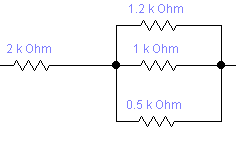
\includegraphics[width=1\textwidth]{authors/stepanuk-2-fig-1.png}
        \caption{Схема к задаче 1}
        \label{fig:stepanuk-2-fig-1}
    \end{minipage}
\hfill
    \begin{minipage}[h]{0.5\linewidth}
        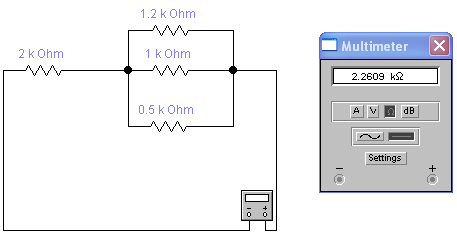
\includegraphics[width=1\textwidth]{authors/stepanuk-2-fig-2.png}
        \caption{Решение задачи 1 в программе}
        \label{fig:stepanuk-2-fig-2}
    \end{minipage}


  \end{center}
\end{changemargin}

\end{figure}




\textbf{Задача 2}. \textit{Определить ток в цепи} (рис.~3).

$$\text{Решение (рис.~4):}\quad I=\frac{17\cdot(1500+300+3000)}{(1500+300)\cdot3000}=0,01511\,\text{А}=15,11\text{мА}$$

\vspace{-16pt}
\begin{figure}[H]
%\begin{changemargin}{-1.5cm}{-2cm}
  \begin{center}
    \begin{minipage}[h]{0.36\linewidth}
        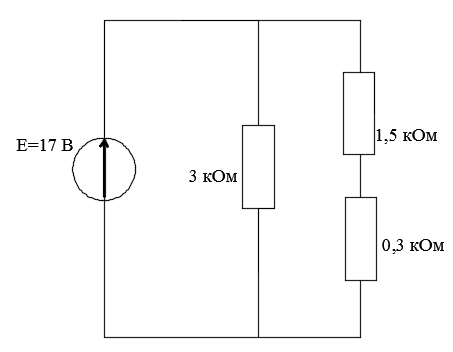
\includegraphics[width=1\textwidth]{authors/stepanuk-2-fig-3.png}
        \caption{Схема к задаче 2}
        \label{fig:stepanuk-2-fig-3}
    \end{minipage}
\hfill
    \begin{minipage}[h]{0.5\linewidth}
        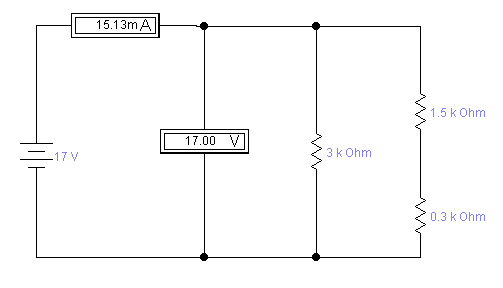
\includegraphics[width=1\textwidth]{authors/stepanuk-2-fig-4.png}
        \caption{Решение задачи 2 в программе}
        \label{fig:stepanuk-2-fig-4}
    \end{minipage}


  \end{center}
%\end{changemargin}

\end{figure}


\textbf{Задача 3}. \textit{Определить токи в ветвях (рис. 5). Проверить правильность их нахождения, используя первый закон Кирхгофа для узла (а).}

Используя принцип наложения находим токи $I_1=8,9, I_2=8,0, I_3=0,9$.

Составим уравнение по первому закону Кирхгофа для узла (а).
\vspace{-6pt}
$$\text{Решение (рис. 6):}\quad I_1=I_2+I_3\Rightarrow8,9=8,0+0,9$$
\vspace{-8pt}
\begin{figure}[H]
%\begin{changemargin}{-1.5cm}{-2cm}
\vspace{-12pt}
  \begin{center}
    \begin{minipage}[h]{0.5\linewidth}
        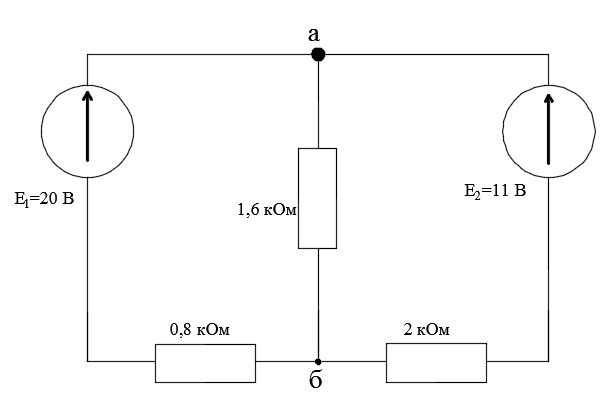
\includegraphics[width=1\textwidth]{authors/stepanuk-2-fig-5.png}
        \caption{Схема к задаче 3}
        \label{fig:stepanuk-2-fig-5}
    \end{minipage}
\hfill
    \begin{minipage}[h]{0.4\linewidth}
        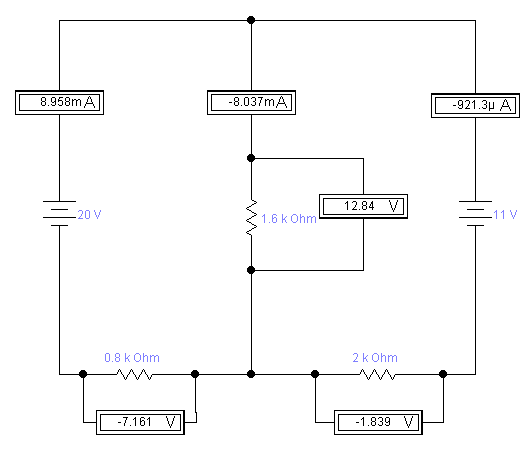
\includegraphics[width=1\textwidth]{authors/stepanuk-2-fig-6.png}
        \caption{Решение задачи 3 в программе}
        \label{fig:stepanuk-2-fig-6}
    \end{minipage}


  \end{center}
%\end{changemargin}
\vspace{-12pt}
\end{figure}

\clearpage

\textbf{Задача 4}. \textit{Определить ток в цепи (рис. 7). Проверить справедливость второго закона Кирхгофа.}
\vspace{-2pt}
$$\text{Решение (рис.~8):}\quad I=\frac{12}{1+0,5+2,4+3,7}=1,58\,\text{А}$$

Запишем уравнение по второму закону Кирхгофа для данного контура.

$$12=(1+0,5+2,4+3,7)\cdot1,58\Rightarrow12=12$$

\begin{figure}[H]
%\begin{changemargin}{-1.5cm}{-2cm}
  \begin{center}
    \begin{minipage}[h]{0.4\linewidth}
        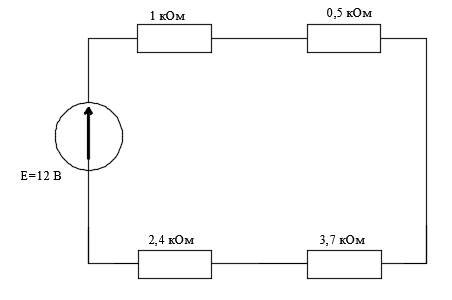
\includegraphics[width=1\textwidth]{authors/stepanuk-2-fig-7.png}
        \caption{Схема к задаче 3}
        \label{fig:stepanuk-2-fig-7}
    \end{minipage}
\hfill
    \begin{minipage}[h]{0.55\linewidth}
        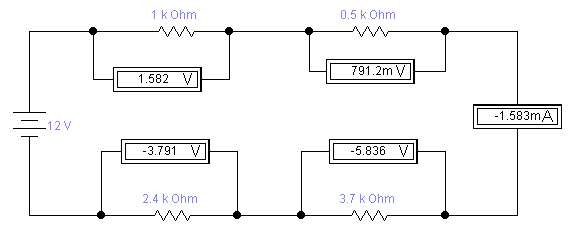
\includegraphics[width=1\textwidth]{authors/stepanuk-2-fig-8.png}
        \caption{Решение задачи 3 в программе}
        \label{fig:stepanuk-2-fig-8}
    \end{minipage}


  \end{center}
%\end{changemargin}

\end{figure}


Практика использования программных комплексов в учебном процессе показывает, повышается качество обучения. За счёт того, что студенты лучше усваивают материал, лучше понимают суть законов и явлений.

Как было сказано ранее программы дополняют и расширяют реальные физические эксперименты, но не могут полностью заменить натурные испытания. В сложившейся эпидемиологической ситуации, когда студенты
находятся на дистанционном обучении виртуальные лаборатории это
единственный способ выполнить учебный план в полном объеме. Развитие
цифровых сервисов в сфере образования будет только нарастать, а уровень
цифровизации будет являться лакмусовой бумагой конкурентоспособности и
привлекательности высшего учебного заведения.

\begin{thebibliography}{99}

\bibitem{}\BibAuthor{Карлащук~В.~И.} Электронная лаборатория на IBM PC. T. 1. Лабораторный практикум на~базе Electronics WorkBench и Matlab.~--- М.~: СолонПресс, 2004.~--- T.~1.~--- 637~с.
\bibitem{}\BibAuthor{Максимов~А.~В.} Использование программного комплекса Electronics Workbench для синтеза и анализа электронных схем и устройств // Материалы XVII межвузовской военно-научной конференции в ЧВИИРЭ.~--- Череповец~: ЧВИИРЭ, 2006.~--- 403~с.
\bibitem{}\BibAuthor{Чернышов~Н.~Г., Чернышова~Т.~И.} Моделирование и анализ схем в Electronics Workbench.~--- Тамбов~: Изд-во Тамб. гос. техн. ун-та, 2005.~--- 52~с.


\end{thebibliography}
